\documentclass[]{article}
\usepackage{lmodern}
\usepackage{amssymb,amsmath}
\usepackage{ifxetex,ifluatex}
\usepackage{fixltx2e} % provides \textsubscript
\ifnum 0\ifxetex 1\fi\ifluatex 1\fi=0 % if pdftex
  \usepackage[T1]{fontenc}
  \usepackage[utf8]{inputenc}
\else % if luatex or xelatex
  \ifxetex
    \usepackage{mathspec}
  \else
    \usepackage{fontspec}
  \fi
  \defaultfontfeatures{Ligatures=TeX,Scale=MatchLowercase}
\fi
% use upquote if available, for straight quotes in verbatim environments
\IfFileExists{upquote.sty}{\usepackage{upquote}}{}
% use microtype if available
\IfFileExists{microtype.sty}{%
\usepackage{microtype}
\UseMicrotypeSet[protrusion]{basicmath} % disable protrusion for tt fonts
}{}
\usepackage[margin=1in]{geometry}
\usepackage{hyperref}
\hypersetup{unicode=true,
            pdftitle={ESM206-assignment4},
            pdfauthor={Claire Madden, Bridget Gibbons, Andrew Paterson},
            pdfborder={0 0 0},
            breaklinks=true}
\urlstyle{same}  % don't use monospace font for urls
\usepackage{color}
\usepackage{fancyvrb}
\newcommand{\VerbBar}{|}
\newcommand{\VERB}{\Verb[commandchars=\\\{\}]}
\DefineVerbatimEnvironment{Highlighting}{Verbatim}{commandchars=\\\{\}}
% Add ',fontsize=\small' for more characters per line
\usepackage{framed}
\definecolor{shadecolor}{RGB}{248,248,248}
\newenvironment{Shaded}{\begin{snugshade}}{\end{snugshade}}
\newcommand{\KeywordTok}[1]{\textcolor[rgb]{0.13,0.29,0.53}{\textbf{#1}}}
\newcommand{\DataTypeTok}[1]{\textcolor[rgb]{0.13,0.29,0.53}{#1}}
\newcommand{\DecValTok}[1]{\textcolor[rgb]{0.00,0.00,0.81}{#1}}
\newcommand{\BaseNTok}[1]{\textcolor[rgb]{0.00,0.00,0.81}{#1}}
\newcommand{\FloatTok}[1]{\textcolor[rgb]{0.00,0.00,0.81}{#1}}
\newcommand{\ConstantTok}[1]{\textcolor[rgb]{0.00,0.00,0.00}{#1}}
\newcommand{\CharTok}[1]{\textcolor[rgb]{0.31,0.60,0.02}{#1}}
\newcommand{\SpecialCharTok}[1]{\textcolor[rgb]{0.00,0.00,0.00}{#1}}
\newcommand{\StringTok}[1]{\textcolor[rgb]{0.31,0.60,0.02}{#1}}
\newcommand{\VerbatimStringTok}[1]{\textcolor[rgb]{0.31,0.60,0.02}{#1}}
\newcommand{\SpecialStringTok}[1]{\textcolor[rgb]{0.31,0.60,0.02}{#1}}
\newcommand{\ImportTok}[1]{#1}
\newcommand{\CommentTok}[1]{\textcolor[rgb]{0.56,0.35,0.01}{\textit{#1}}}
\newcommand{\DocumentationTok}[1]{\textcolor[rgb]{0.56,0.35,0.01}{\textbf{\textit{#1}}}}
\newcommand{\AnnotationTok}[1]{\textcolor[rgb]{0.56,0.35,0.01}{\textbf{\textit{#1}}}}
\newcommand{\CommentVarTok}[1]{\textcolor[rgb]{0.56,0.35,0.01}{\textbf{\textit{#1}}}}
\newcommand{\OtherTok}[1]{\textcolor[rgb]{0.56,0.35,0.01}{#1}}
\newcommand{\FunctionTok}[1]{\textcolor[rgb]{0.00,0.00,0.00}{#1}}
\newcommand{\VariableTok}[1]{\textcolor[rgb]{0.00,0.00,0.00}{#1}}
\newcommand{\ControlFlowTok}[1]{\textcolor[rgb]{0.13,0.29,0.53}{\textbf{#1}}}
\newcommand{\OperatorTok}[1]{\textcolor[rgb]{0.81,0.36,0.00}{\textbf{#1}}}
\newcommand{\BuiltInTok}[1]{#1}
\newcommand{\ExtensionTok}[1]{#1}
\newcommand{\PreprocessorTok}[1]{\textcolor[rgb]{0.56,0.35,0.01}{\textit{#1}}}
\newcommand{\AttributeTok}[1]{\textcolor[rgb]{0.77,0.63,0.00}{#1}}
\newcommand{\RegionMarkerTok}[1]{#1}
\newcommand{\InformationTok}[1]{\textcolor[rgb]{0.56,0.35,0.01}{\textbf{\textit{#1}}}}
\newcommand{\WarningTok}[1]{\textcolor[rgb]{0.56,0.35,0.01}{\textbf{\textit{#1}}}}
\newcommand{\AlertTok}[1]{\textcolor[rgb]{0.94,0.16,0.16}{#1}}
\newcommand{\ErrorTok}[1]{\textcolor[rgb]{0.64,0.00,0.00}{\textbf{#1}}}
\newcommand{\NormalTok}[1]{#1}
\usepackage{graphicx,grffile}
\makeatletter
\def\maxwidth{\ifdim\Gin@nat@width>\linewidth\linewidth\else\Gin@nat@width\fi}
\def\maxheight{\ifdim\Gin@nat@height>\textheight\textheight\else\Gin@nat@height\fi}
\makeatother
% Scale images if necessary, so that they will not overflow the page
% margins by default, and it is still possible to overwrite the defaults
% using explicit options in \includegraphics[width, height, ...]{}
\setkeys{Gin}{width=\maxwidth,height=\maxheight,keepaspectratio}
\IfFileExists{parskip.sty}{%
\usepackage{parskip}
}{% else
\setlength{\parindent}{0pt}
\setlength{\parskip}{6pt plus 2pt minus 1pt}
}
\setlength{\emergencystretch}{3em}  % prevent overfull lines
\providecommand{\tightlist}{%
  \setlength{\itemsep}{0pt}\setlength{\parskip}{0pt}}
\setcounter{secnumdepth}{0}
% Redefines (sub)paragraphs to behave more like sections
\ifx\paragraph\undefined\else
\let\oldparagraph\paragraph
\renewcommand{\paragraph}[1]{\oldparagraph{#1}\mbox{}}
\fi
\ifx\subparagraph\undefined\else
\let\oldsubparagraph\subparagraph
\renewcommand{\subparagraph}[1]{\oldsubparagraph{#1}\mbox{}}
\fi

%%% Use protect on footnotes to avoid problems with footnotes in titles
\let\rmarkdownfootnote\footnote%
\def\footnote{\protect\rmarkdownfootnote}

%%% Change title format to be more compact
\usepackage{titling}

% Create subtitle command for use in maketitle
\newcommand{\subtitle}[1]{
  \posttitle{
    \begin{center}\large#1\end{center}
    }
}

\setlength{\droptitle}{-2em}

  \title{ESM206-assignment4}
    \pretitle{\vspace{\droptitle}\centering\huge}
  \posttitle{\par}
    \author{Claire Madden, Bridget Gibbons, Andrew Paterson}
    \preauthor{\centering\large\emph}
  \postauthor{\par}
      \predate{\centering\large\emph}
  \postdate{\par}
    \date{11/12/2018}

\usepackage{booktabs}
\usepackage{longtable}
\usepackage{array}
\usepackage{multirow}
\usepackage[table]{xcolor}
\usepackage{wrapfig}
\usepackage{float}
\usepackage{colortbl}
\usepackage{pdflscape}
\usepackage{tabu}
\usepackage{threeparttable}
\usepackage{threeparttablex}
\usepackage[normalem]{ulem}
\usepackage{makecell}

\begin{document}
\maketitle

\begin{Shaded}
\begin{Highlighting}[]
\NormalTok{lobster_size2 <-}\StringTok{ }\KeywordTok{as.data.frame}\NormalTok{(lobster_size)}
\NormalTok{lobster_size_tidy <-}\StringTok{ }\KeywordTok{expand.dft}\NormalTok{(lobster_size2, }\DataTypeTok{freq =} \StringTok{"COUNT"}\NormalTok{)}

\CommentTok{#If you guys don't want to change the site name here, no problem!}
\NormalTok{size_tidy <-}\StringTok{ }\NormalTok{lobster_size_tidy }\OperatorTok\StringTok{ }
\StringTok{  }\KeywordTok{mutate}\NormalTok{(}\DataTypeTok{Site=}
    \KeywordTok{case_when}\NormalTok{(}
\NormalTok{      SITE }\OperatorTok{==}\StringTok{ "NAPL"} \OperatorTok{~}\StringTok{ "Naples Reef"}\NormalTok{,}
\NormalTok{      SITE }\OperatorTok{==}\StringTok{ "AQUE"} \OperatorTok{~}\StringTok{ "Arroyo Quemado"}\NormalTok{,}
\NormalTok{      SITE }\OperatorTok{==}\StringTok{ "MOHK"} \OperatorTok{~}\StringTok{ "Mohawk Reef"}\NormalTok{,}
\NormalTok{      SITE }\OperatorTok{==}\StringTok{ "IVEE"} \OperatorTok{~}\StringTok{ "Isla Vista"}\NormalTok{,}
\NormalTok{      SITE }\OperatorTok{==}\StringTok{ "CARP"} \OperatorTok{~}\StringTok{ "Carpinteria"}
\NormalTok{    )}
\NormalTok{  ) }\OperatorTok\StringTok{ }
\StringTok{  }\KeywordTok{select}\NormalTok{(}\OperatorTok{-}\NormalTok{SITE)}

\NormalTok{traps_tidy <-}\StringTok{ }\NormalTok{lobster_traps }\OperatorTok\StringTok{ }
\StringTok{    }\KeywordTok{mutate}\NormalTok{(}\DataTypeTok{Site=}
    \KeywordTok{case_when}\NormalTok{(}
\NormalTok{      SITE }\OperatorTok{==}\StringTok{ "NAPL"} \OperatorTok{~}\StringTok{ "Naples Reef"}\NormalTok{,}
\NormalTok{      SITE }\OperatorTok{==}\StringTok{ "AQUE"} \OperatorTok{~}\StringTok{ "Arroyo Quemado"}\NormalTok{,}
\NormalTok{      SITE }\OperatorTok{==}\StringTok{ "MOHK"} \OperatorTok{~}\StringTok{ "Mohawk Reef"}\NormalTok{,}
\NormalTok{      SITE }\OperatorTok{==}\StringTok{ "IVEE"} \OperatorTok{~}\StringTok{ "Isla Vista"}\NormalTok{,}
\NormalTok{      SITE }\OperatorTok{==}\StringTok{ "CARP"} \OperatorTok{~}\StringTok{ "Carpinteria"}
\NormalTok{    )}
\NormalTok{  ) }\OperatorTok\StringTok{ }
\StringTok{  }\KeywordTok{select}\NormalTok{(}\OperatorTok{-}\NormalTok{SITE)}
\end{Highlighting}
\end{Shaded}

\section{Part 1 (Claire)}\label{part-1-claire}

\begin{Shaded}
\begin{Highlighting}[]
\NormalTok{abundance_summary <-}\StringTok{ }\NormalTok{lobster_size }\OperatorTok
\StringTok{  }\KeywordTok{group_by}\NormalTok{(SITE, YEAR) }\OperatorTok\StringTok{ }
\StringTok{  }\KeywordTok{summarize}\NormalTok{(}
    \DataTypeTok{count =} \KeywordTok{sum}\NormalTok{(COUNT))}

\NormalTok{abundance_column <-}\StringTok{ }\KeywordTok{ggplot}\NormalTok{(abundance_summary, }\KeywordTok{aes}\NormalTok{( }\DataTypeTok{x =}\NormalTok{ YEAR, }\DataTypeTok{y =}\NormalTok{ count))}\OperatorTok{+}
\StringTok{  }\KeywordTok{geom_col}\NormalTok{()}\OperatorTok{+}
\StringTok{  }\KeywordTok{facet_wrap}\NormalTok{(}\OperatorTok{~}\NormalTok{SITE)}

\NormalTok{abundance_column}
\end{Highlighting}
\end{Shaded}

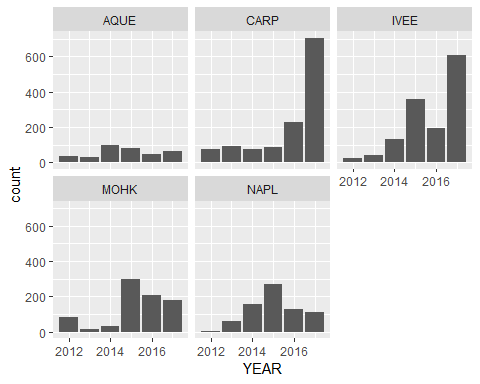
\includegraphics{ESM206-assignment4_files/figure-latex/unnamed-chunk-4-1.pdf}

\begin{Shaded}
\begin{Highlighting}[]
\NormalTok{traps_simple <-}\StringTok{ }\NormalTok{lobster_traps }\OperatorTok\StringTok{ }
\StringTok{  }\KeywordTok{filter}\NormalTok{(SITE }\OperatorTok{==}\StringTok{ "AQUE"} \OperatorTok{|}\StringTok{ }\NormalTok{SITE }\OperatorTok{==}\StringTok{ "NAPL"} \OperatorTok{|}\StringTok{ }\NormalTok{SITE }\OperatorTok{==}\StringTok{ "MOHK"} \OperatorTok{|}\StringTok{ }\NormalTok{SITE }\OperatorTok{==}\StringTok{ "IVEE"} \OperatorTok{|}\StringTok{ }\NormalTok{SITE }\OperatorTok{==}\StringTok{ "CARP"}\NormalTok{)}

\NormalTok{traps_summary <-}\StringTok{ }\NormalTok{traps_simple }\OperatorTok\StringTok{ }
\StringTok{  }\KeywordTok{group_by}\NormalTok{(SITE, YEAR) }\OperatorTok\StringTok{ }
\StringTok{  }\KeywordTok{summarize}\NormalTok{(}
    \DataTypeTok{traps =} \KeywordTok{sum}\NormalTok{(TRAPS))}

\NormalTok{traps_column <-}\StringTok{ }\KeywordTok{ggplot}\NormalTok{(traps_summary, }\KeywordTok{aes}\NormalTok{( }\DataTypeTok{x =}\NormalTok{ YEAR, }\DataTypeTok{y =}\NormalTok{ traps))}\OperatorTok{+}
\StringTok{  }\KeywordTok{geom_col}\NormalTok{()}\OperatorTok{+}
\StringTok{  }\KeywordTok{facet_wrap}\NormalTok{(}\OperatorTok{~}\NormalTok{SITE)}

\NormalTok{traps_column}
\end{Highlighting}
\end{Shaded}

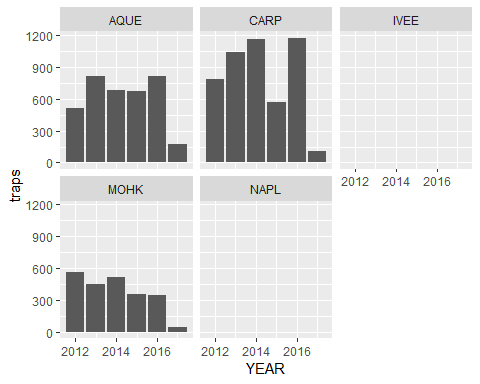
\includegraphics{ESM206-assignment4_files/figure-latex/unnamed-chunk-4-2.pdf}

\begin{Shaded}
\begin{Highlighting}[]
\NormalTok{abundance_scatter <-}\StringTok{ }\KeywordTok{ggplot}\NormalTok{(abundance_summary, }\KeywordTok{aes}\NormalTok{(}\DataTypeTok{x =}\NormalTok{ YEAR, }\DataTypeTok{y =}\NormalTok{ count))}\OperatorTok{+}
\StringTok{  }\KeywordTok{geom_point}\NormalTok{()}\OperatorTok{+}
\StringTok{  }\KeywordTok{geom_line}\NormalTok{()}\OperatorTok{+}
\StringTok{  }\KeywordTok{facet_wrap}\NormalTok{(}\OperatorTok{~}\NormalTok{SITE)}

\NormalTok{abundance_scatter}
\end{Highlighting}
\end{Shaded}

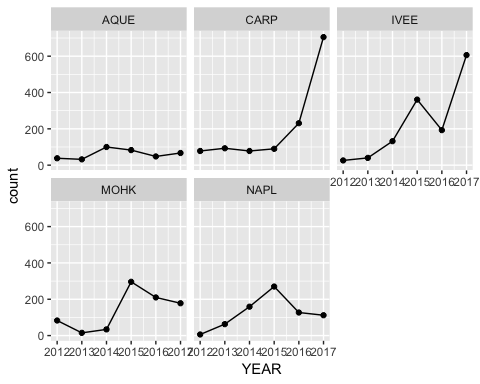
\includegraphics{ESM206-assignment4_files/figure-latex/unnamed-chunk-4-3.pdf}

\begin{Shaded}
\begin{Highlighting}[]
\NormalTok{traps_scatter <-}\StringTok{ }\KeywordTok{ggplot}\NormalTok{(traps_summary, }\KeywordTok{aes}\NormalTok{(}\DataTypeTok{x =}\NormalTok{ YEAR, }\DataTypeTok{y =}\NormalTok{ traps))}\OperatorTok{+}
\StringTok{  }\KeywordTok{geom_point}\NormalTok{()}\OperatorTok{+}
\StringTok{  }\KeywordTok{geom_line}\NormalTok{()}\OperatorTok{+}
\StringTok{  }\KeywordTok{facet_wrap}\NormalTok{(}\OperatorTok{~}\NormalTok{SITE)}

\NormalTok{traps_scatter}
\end{Highlighting}
\end{Shaded}

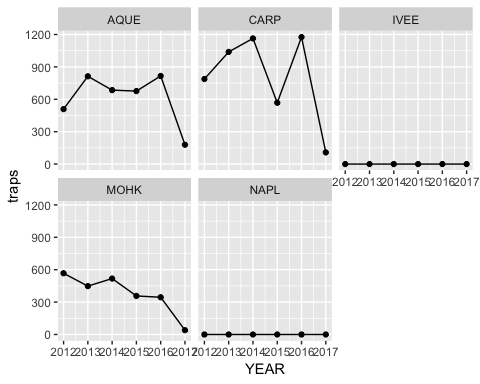
\includegraphics{ESM206-assignment4_files/figure-latex/unnamed-chunk-4-4.pdf}

\begin{Shaded}
\begin{Highlighting}[]
\CommentTok{# my attempt at joining the data before graphing and or getting both graphs for one location on the same plane}

\NormalTok{abundance_traps <-}\StringTok{ }\KeywordTok{full_join}\NormalTok{(abundance_summary, traps_summary)}
\end{Highlighting}
\end{Shaded}

\begin{verbatim}
## Joining, by = c("SITE", "YEAR")
\end{verbatim}

\begin{Shaded}
\begin{Highlighting}[]
\NormalTok{both_scatter <-}\StringTok{ }\KeywordTok{ggplot}\NormalTok{(abundance_traps, }\KeywordTok{aes}\NormalTok{(}\DataTypeTok{x =}\NormalTok{ YEAR))}\OperatorTok{+}
\StringTok{  }\KeywordTok{geom_line}\NormalTok{(}\KeywordTok{aes}\NormalTok{(}\DataTypeTok{y=}\NormalTok{count, }\DataTypeTok{color =} \StringTok{"blue"}\NormalTok{))}\OperatorTok{+}
\StringTok{  }\KeywordTok{geom_line}\NormalTok{(}\KeywordTok{aes}\NormalTok{(}\DataTypeTok{y=}\NormalTok{traps, }\DataTypeTok{color =} \StringTok{"red"}\NormalTok{))}\OperatorTok{+}
\StringTok{  }\KeywordTok{facet_wrap}\NormalTok{(}\OperatorTok{~}\NormalTok{SITE)}\OperatorTok{+}
\StringTok{  }\KeywordTok{theme_light}\NormalTok{()}

\NormalTok{both_scatter}
\end{Highlighting}
\end{Shaded}

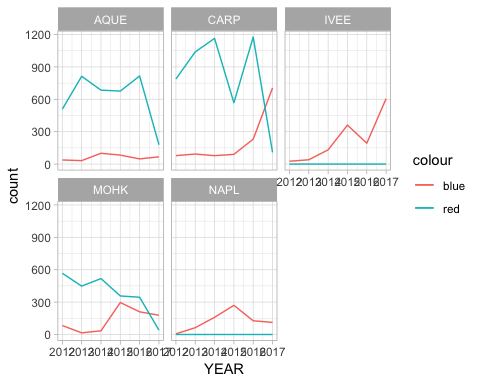
\includegraphics{ESM206-assignment4_files/figure-latex/unnamed-chunk-5-1.pdf}

\section{Part 2 (Andrew)}\label{part-2-andrew}

\begin{Shaded}
\begin{Highlighting}[]
\CommentTok{#Filter for just 2017 results for Part 2, and Exploratory Histogram and QQ Plots}

\NormalTok{size_}\DecValTok{2017}\NormalTok{ <-}\StringTok{ }\NormalTok{size_tidy }\OperatorTok\StringTok{ }
\StringTok{  }\KeywordTok{filter}\NormalTok{(YEAR }\OperatorTok{==}\StringTok{ "2017"}\NormalTok{) }\OperatorTok
\StringTok{  }\KeywordTok{select}\NormalTok{(SIZE, Site)}

\NormalTok{carapace_hist <-}\StringTok{ }\KeywordTok{ggplot}\NormalTok{(size_}\DecValTok{2017}\NormalTok{, }\KeywordTok{aes}\NormalTok{(}\DataTypeTok{x =}\NormalTok{ SIZE))}\OperatorTok{+}
\StringTok{  }\KeywordTok{geom_histogram}\NormalTok{(}\DataTypeTok{bins =} \DecValTok{23}\NormalTok{, }\KeywordTok{aes}\NormalTok{(}\DataTypeTok{fill =}\NormalTok{ Site))}\OperatorTok{+}
\StringTok{  }\KeywordTok{facet_wrap}\NormalTok{(}\OperatorTok{~}\NormalTok{Site)}

\NormalTok{carapace_hist}
\end{Highlighting}
\end{Shaded}

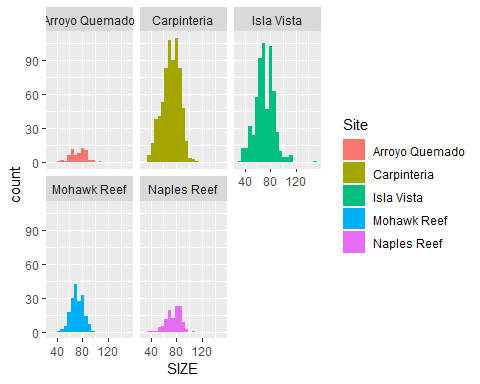
\includegraphics{ESM206-assignment4_files/figure-latex/unnamed-chunk-6-1.pdf}

\begin{Shaded}
\begin{Highlighting}[]
\NormalTok{carapace_qq <-}\StringTok{ }\KeywordTok{ggplot}\NormalTok{(size_}\DecValTok{2017}\NormalTok{, }\KeywordTok{aes}\NormalTok{(}\DataTypeTok{sample =}\NormalTok{ SIZE))}\OperatorTok{+}
\StringTok{  }\KeywordTok{geom_qq}\NormalTok{()}\OperatorTok{+}
\StringTok{  }\KeywordTok{facet_wrap}\NormalTok{(}\OperatorTok{~}\NormalTok{Site)}

\NormalTok{carapace_qq}
\end{Highlighting}
\end{Shaded}

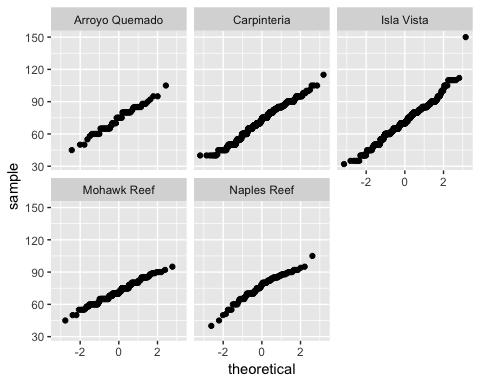
\includegraphics{ESM206-assignment4_files/figure-latex/unnamed-chunk-6-2.pdf}

\begin{Shaded}
\begin{Highlighting}[]
\CommentTok{#The data looks roughly normally distributed, and all sites have a sample size of greater than 30. }
\end{Highlighting}
\end{Shaded}

\begin{Shaded}
\begin{Highlighting}[]
\CommentTok{#Levene's Test for Equal Variances, since we have more than two groups}
\CommentTok{#H0: Variances are equal}
\CommentTok{#HA: Variances are not equal}

\NormalTok{carapace_levene <-}\StringTok{ }\KeywordTok{leveneTest}\NormalTok{(SIZE }\OperatorTok{~}\StringTok{ }\NormalTok{Site, }\DataTypeTok{data =}\NormalTok{ size_}\DecValTok{2017}\NormalTok{)}
\end{Highlighting}
\end{Shaded}

\begin{verbatim}
## Warning in leveneTest.default(y = y, group = group, ...): group coerced to
## factor.
\end{verbatim}

\begin{Shaded}
\begin{Highlighting}[]
\NormalTok{carapace_levene}
\end{Highlighting}
\end{Shaded}

\begin{verbatim}
## Levene's Test for Homogeneity of Variance (center = median)
##         Df F value    Pr(>F)    
## group    4  8.3893 1.065e-06 ***
##       1663                      
## ---
## Signif. codes:  0 '***' 0.001 '**' 0.01 '*' 0.05 '.' 0.1 ' ' 1
\end{verbatim}

\begin{Shaded}
\begin{Highlighting}[]
\CommentTok{#We reject the null hypothesis of equal variances (p < .001) based on Levene's Test.  However, we can examine the variances of each site to see if the largest is less than four times the smallest variance.  }

\NormalTok{carapace_variances <-}\StringTok{ }\NormalTok{size_}\DecValTok{2017} \OperatorTok\StringTok{ }
\StringTok{  }\KeywordTok{group_by}\NormalTok{(Site) }\OperatorTok\StringTok{ }
\StringTok{  }\KeywordTok{summarize}\NormalTok{(}
    \DataTypeTok{Variance =} \KeywordTok{var}\NormalTok{(SIZE)}
\NormalTok{  )}

\NormalTok{carapace_variances}
\end{Highlighting}
\end{Shaded}

\begin{verbatim}
## # A tibble: 5 x 2
##   Site           Variance
##   <chr>             <dbl>
## 1 Arroyo Quemado    141. 
## 2 Carpinteria       174. 
## 3 Isla Vista        205. 
## 4 Mohawk Reef        86.1
## 5 Naples Reef       130.
\end{verbatim}

\begin{Shaded}
\begin{Highlighting}[]
\CommentTok{#The largest variance is well less than four times the smallest variance, so we can assume accept the null hypothesis of equal variances and run an ANOVA.}

\CommentTok{#H0: Mean carapace sizes are equal at all sites}
\CommentTok{#HA: Mean carapace sizes vary for lobsters from at least two sites.}

\NormalTok{carapace_aov <-}\StringTok{ }\KeywordTok{aov}\NormalTok{(SIZE }\OperatorTok{~}\StringTok{ }\NormalTok{Site, }\DataTypeTok{data =}\NormalTok{ size_}\DecValTok{2017}\NormalTok{)}
\KeywordTok{summary}\NormalTok{(carapace_aov)}
\end{Highlighting}
\end{Shaded}

\begin{verbatim}
##               Df Sum Sq Mean Sq F value Pr(>F)   
## Site           4   2355   588.6   3.424 0.0085 **
## Residuals   1663 285871   171.9                  
## ---
## Signif. codes:  0 '***' 0.001 '**' 0.01 '*' 0.05 '.' 0.1 ' ' 1
\end{verbatim}

\begin{Shaded}
\begin{Highlighting}[]
\CommentTok{#boxplot for ANOVA in case we want to include this}
\NormalTok{lobster_anova <-}\StringTok{ }\KeywordTok{ggplot}\NormalTok{(size_}\DecValTok{2017}\NormalTok{, }\KeywordTok{aes}\NormalTok{(}\DataTypeTok{x =}\NormalTok{ Site, }\DataTypeTok{y =}\NormalTok{ SIZE))}\OperatorTok{+}
\StringTok{  }\KeywordTok{geom_boxplot}\NormalTok{()}\OperatorTok{+}
\StringTok{  }\KeywordTok{scale_x_discrete}\NormalTok{()}\OperatorTok{+}
\StringTok{  }\KeywordTok{scale_y_discrete}\NormalTok{()}\OperatorTok{+}
\StringTok{  }\KeywordTok{ylab}\NormalTok{(}\StringTok{"Size"}\NormalTok{)}\OperatorTok{+}
\StringTok{  }\KeywordTok{xlab}\NormalTok{(}\StringTok{"Site"}\NormalTok{)}

\NormalTok{lobster_anova}
\end{Highlighting}
\end{Shaded}

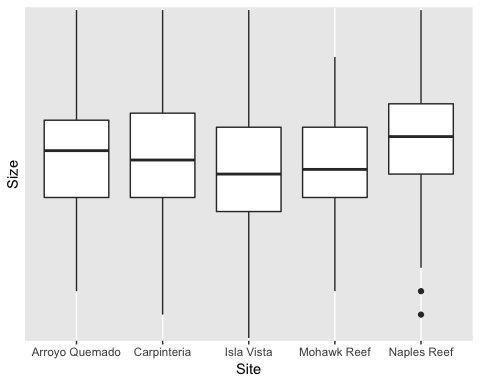
\includegraphics{ESM206-assignment4_files/figure-latex/unnamed-chunk-7-1.pdf}

\begin{Shaded}
\begin{Highlighting}[]
\CommentTok{#With p = .0085, we reject the null, and assume mean carapace length varies between lobsters from at least two sites. At least two populations were taken from populations with different means.}

\CommentTok{#Post-hoc testing using Tukey's HSD}

\NormalTok{carapace_ph <-}\StringTok{ }\KeywordTok{TukeyHSD}\NormalTok{(carapace_aov)}
\NormalTok{carapace_ph}
\end{Highlighting}
\end{Shaded}

\begin{verbatim}
##   Tukey multiple comparisons of means
##     95% family-wise confidence level
## 
## Fit: aov(formula = SIZE ~ Site, data = size_2017)
## 
## $Site
##                                  diff         lwr      upr     p adj
## Carpinteria-Arroyo Quemado -1.6657352 -6.24294710 2.911477 0.8582355
## Isla Vista-Arroyo Quemado  -2.4433772 -7.05292315 2.166169 0.5968998
## Mohawk Reef-Arroyo Quemado -1.8955224 -7.02720717 3.236162 0.8514711
## Naples Reef-Arroyo Quemado  2.3366205 -3.19311600 7.866357 0.7775633
## Isla Vista-Carpinteria     -0.7776420 -2.76097123 1.205687 0.8216104
## Mohawk Reef-Carpinteria    -0.2297872 -3.23309697 2.773523 0.9995765
## Naples Reef-Carpinteria     4.0023556  0.36042398 7.644287 0.0228728
## Mohawk Reef-Isla Vista      0.5478548 -2.50450730 3.600217 0.9882889
## Naples Reef-Isla Vista      4.7799976  1.09751057 8.462485 0.0037001
## Naples Reef-Mohawk Reef     4.2321429 -0.08607271 8.550358 0.0579286
\end{verbatim}

\begin{Shaded}
\begin{Highlighting}[]
\CommentTok{#Lobster sizes differed significantly only between Naples Reef and Carpenteria, and Naples Reef and Isla Vista. Do we want to run Cohen's d here?  It might get very clunky to convey all of the effect sizes, or maybe we could make a table showing all of the differences and effect sizes?}
\end{Highlighting}
\end{Shaded}

\textbf{Figure 1: Mean Lobster Carapace Length at Five LTER Sites in the
Santa Barbara Channel}

\begin{Shaded}
\begin{Highlighting}[]
\CommentTok{#Comparing the lobster sizes across the sites, and putting this information in a table.}

\NormalTok{size_summary <-}\StringTok{ }\NormalTok{size_}\DecValTok{2017} \OperatorTok\StringTok{ }
\StringTok{  }\KeywordTok{group_by}\NormalTok{(Site) }\OperatorTok\StringTok{ }
\StringTok{  }\KeywordTok{summarize}\NormalTok{(}\StringTok{"Mean Size"}\NormalTok{ =}\StringTok{ }\KeywordTok{round}\NormalTok{(}\KeywordTok{mean}\NormalTok{(SIZE), }\DecValTok{2}\NormalTok{),}
            \StringTok{"Sample Size"}\NormalTok{ =}\StringTok{ }\KeywordTok{length}\NormalTok{(Site))}

\NormalTok{size_summary}
\end{Highlighting}
\end{Shaded}

\begin{verbatim}
## # A tibble: 5 x 3
##   Site           `Mean Size` `Sample Size`
##   <chr>                <dbl>         <int>
## 1 Arroyo Quemado        73.9            67
## 2 Carpinteria           72.2           705
## 3 Isla Vista            71.4           606
## 4 Mohawk Reef           72             178
## 5 Naples Reef           76.2           112
\end{verbatim}

\begin{Shaded}
\begin{Highlighting}[]
\NormalTok{size_final <-}\StringTok{ }\KeywordTok{kable}\NormalTok{(size_summary, }\DataTypeTok{col.names =} \KeywordTok{c}\NormalTok{(}\StringTok{"Site"}\NormalTok{, }\StringTok{"Mean Carapace Size (mm)"}\NormalTok{, }\StringTok{"Sample Size"}\NormalTok{), }\DataTypeTok{align =} \StringTok{"c"}\NormalTok{) }\OperatorTok\StringTok{ }
\StringTok{  }\KeywordTok{kable_styling}\NormalTok{(}\DataTypeTok{bootstrap_options =} \KeywordTok{c}\NormalTok{(}\StringTok{"striped"}\NormalTok{))}

\NormalTok{size_final}
\end{Highlighting}
\end{Shaded}

\begin{table}[H]
\centering
\begin{tabular}{c|c|c}
\hline
Site & Mean Carapace Size (mm) & Sample Size\\
\hline
Arroyo Quemado & 73.90 & 67\\
\hline
Carpinteria & 72.23 & 705\\
\hline
Isla Vista & 71.45 & 606\\
\hline
Mohawk Reef & 72.00 & 178\\
\hline
Naples Reef & 76.23 & 112\\
\hline
\end{tabular}
\end{table}

\section{Part 3 (Bridget)}\label{part-3-bridget}

\subsection{These chunks are lumping all the MPV sites together and then
comparing 2012 and 2017, and then doing the same thing for non-MPV
sites. If we need to do it site by site, this all needs to be
changed}\label{these-chunks-are-lumping-all-the-mpv-sites-together-and-then-comparing-2012-and-2017-and-then-doing-the-same-thing-for-non-mpv-sites.-if-we-need-to-do-it-site-by-site-this-all-needs-to-be-changed}

\section{MPA sites: Isla Vista, Naples
Reef}\label{mpa-sites-isla-vista-naples-reef}

\section{Non-MPA sites:Arroyo Quemado, Carpinteria, Mohawk
Reef}\label{non-mpa-sitesarroyo-quemado-carpinteria-mohawk-reef}

\begin{Shaded}
\begin{Highlighting}[]
\CommentTok{#For the MPA sites}

\NormalTok{mpa_size <-}\StringTok{ }\NormalTok{lobster_size_tidy }\OperatorTok\StringTok{ }
\StringTok{  }\KeywordTok{filter}\NormalTok{(SITE }\OperatorTok{==}\StringTok{ "IVEE"} \OperatorTok{|}\StringTok{ }\NormalTok{SITE }\OperatorTok{==}\StringTok{ "NAPL"}\NormalTok{) }\OperatorTok\StringTok{ }
\StringTok{  }\KeywordTok{filter}\NormalTok{(YEAR }\OperatorTok{==}\StringTok{ "2012"} \OperatorTok{|}\StringTok{ }\NormalTok{YEAR }\OperatorTok{==}\StringTok{ "2017"}\NormalTok{) }\OperatorTok\StringTok{ }
\StringTok{  }\KeywordTok{select}\NormalTok{(YEAR, SIZE)}
  
  
\CommentTok{#Need to test for normality to determine which kind of test to run}

\NormalTok{mpa_size_hist <-}\StringTok{ }\KeywordTok{ggplot}\NormalTok{(mpa_size, }\KeywordTok{aes}\NormalTok{(}\DataTypeTok{x =}\NormalTok{ SIZE)) }\OperatorTok{+}\StringTok{ }
\StringTok{  }\KeywordTok{geom_histogram}\NormalTok{(}\DataTypeTok{bins =} \DecValTok{8}\NormalTok{) }\OperatorTok{+}
\StringTok{  }\KeywordTok{facet_wrap}\NormalTok{(}\OperatorTok{~}\NormalTok{YEAR, }\DataTypeTok{scale =} \StringTok{"free"}\NormalTok{)}
  
\NormalTok{mpa_size_hist}
\end{Highlighting}
\end{Shaded}

\includegraphics{ESM206-assignment4_files/figure-latex/unnamed-chunk-9-1.pdf}

\begin{Shaded}
\begin{Highlighting}[]
\NormalTok{mpa_size_qq <-}\StringTok{ }\KeywordTok{ggplot}\NormalTok{ (mpa_size, }\KeywordTok{aes}\NormalTok{(}\DataTypeTok{sample =}\NormalTok{ SIZE)) }\OperatorTok{+}
\StringTok{  }\KeywordTok{geom_qq}\NormalTok{() }\OperatorTok{+}
\StringTok{  }\KeywordTok{facet_wrap}\NormalTok{(}\OperatorTok{~}\NormalTok{YEAR)}

\NormalTok{mpa_size_qq}
\end{Highlighting}
\end{Shaded}

\includegraphics{ESM206-assignment4_files/figure-latex/unnamed-chunk-9-2.pdf}

\begin{Shaded}
\begin{Highlighting}[]
\CommentTok{#The data for 2017 looks normally distributed, but the qq plot for 2012 doesn't look linear. We have more than 30 samples for each year though so we can still use a t-test}

\NormalTok{mpa_}\DecValTok{2012}\NormalTok{ <-}\StringTok{ }\NormalTok{mpa_size }\OperatorTok\StringTok{ }
\StringTok{  }\KeywordTok{filter}\NormalTok{(YEAR }\OperatorTok{==}\StringTok{ "2012"}\NormalTok{) }\OperatorTok\StringTok{ }
\StringTok{  }\KeywordTok{pull}\NormalTok{(SIZE)}

\NormalTok{mpa_}\DecValTok{2017}\NormalTok{ <-}\StringTok{ }\NormalTok{mpa_size }\OperatorTok\StringTok{ }
\StringTok{  }\KeywordTok{filter}\NormalTok{(YEAR }\OperatorTok{==}\StringTok{ "2017"}\NormalTok{) }\OperatorTok\StringTok{ }
\StringTok{  }\KeywordTok{pull}\NormalTok{(SIZE)}

\CommentTok{#Run an F-test to see which type of t-test we can use}
\CommentTok{#H0: ratio of variances is equal to 1}
\CommentTok{#HA: ratio of variances is NOT equal to 1}

\NormalTok{mpa_ftest <-}\StringTok{ }\KeywordTok{var.test}\NormalTok{(mpa_}\DecValTok{2012}\NormalTok{, mpa_}\DecValTok{2017}\NormalTok{)}
\NormalTok{mpa_ftest}
\end{Highlighting}
\end{Shaded}

\begin{verbatim}
## 
##  F test to compare two variances
## 
## data:  mpa_2012 and mpa_2017
## F = 0.75323, num df = 31, denom df = 717, p-value = 0.3346
## alternative hypothesis: true ratio of variances is not equal to 1
## 95 percent confidence interval:
##  0.477719 1.341900
## sample estimates:
## ratio of variances 
##          0.7532319
\end{verbatim}

\begin{Shaded}
\begin{Highlighting}[]
\CommentTok{#Based on result of F-test (p = 0.3346), we retain null hypothesis that variances are equal. We can use a student's t-test, which is more powerful than a Welch's test}

\CommentTok{#H0 - difference in means is 0}
\CommentTok{#HA - difference in means is NOT 0}

\NormalTok{mpa_ttest <-}\StringTok{ }\KeywordTok{t.test}\NormalTok{(mpa_}\DecValTok{2012}\NormalTok{, mpa_}\DecValTok{2017}\NormalTok{, }\DataTypeTok{var.equal =} \OtherTok{TRUE}\NormalTok{)}
\NormalTok{mpa_ttest}
\end{Highlighting}
\end{Shaded}

\begin{verbatim}
## 
##  Two Sample t-test
## 
## data:  mpa_2012 and mpa_2017
## t = -1.9159, df = 748, p-value = 0.05576
## alternative hypothesis: true difference in means is not equal to 0
## 95 percent confidence interval:
##  -9.7644724  0.1189292
## sample estimates:
## mean of x mean of y 
##  67.37500  72.19777
\end{verbatim}

\begin{Shaded}
\begin{Highlighting}[]
\CommentTok{#With p-value of 0.05576, we retain null hypothesis. There is not a significant difference in mean lobster size in MPAs between 2012 and 2017.}

\CommentTok{#Calculate effect size}

\NormalTok{mpa_eff_size <-}\StringTok{ }\KeywordTok{cohen.d}\NormalTok{(mpa_}\DecValTok{2012}\NormalTok{, mpa_}\DecValTok{2017}\NormalTok{)}
\NormalTok{mpa_eff_size}
\end{Highlighting}
\end{Shaded}

\begin{verbatim}
## 
## Cohen's d
## 
## d estimate: -0.3461506 (small)
## 95 percent confidence interval:
##          inf          sup 
## -0.701270908  0.008969759
\end{verbatim}

\begin{Shaded}
\begin{Highlighting}[]
\CommentTok{#There is a small effect size (-0.34)}
\end{Highlighting}
\end{Shaded}

\begin{Shaded}
\begin{Highlighting}[]
\CommentTok{#Boxplot for MPA}
\NormalTok{mpa_size_ordered <-}\StringTok{ }\NormalTok{mpa_size }\OperatorTok\StringTok{ }
\StringTok{  }\KeywordTok{mutate}\NormalTok{(}\DataTypeTok{YEAR =} \KeywordTok{factor}\NormalTok{(YEAR)) }\OperatorTok\StringTok{ }
\StringTok{  }\KeywordTok{group_by}\NormalTok{(YEAR)}

\NormalTok{mpa_size_boxplot <-}\StringTok{ }\KeywordTok{ggplot}\NormalTok{(mpa_size_ordered, }\KeywordTok{aes}\NormalTok{(}\DataTypeTok{x =}\NormalTok{ YEAR, }\DataTypeTok{y =}\NormalTok{ SIZE)) }\OperatorTok{+}
\StringTok{  }\KeywordTok{geom_boxplot}\NormalTok{()}

\NormalTok{mpa_size_boxplot}
\end{Highlighting}
\end{Shaded}

\includegraphics{ESM206-assignment4_files/figure-latex/unnamed-chunk-10-1.pdf}

\begin{Shaded}
\begin{Highlighting}[]
\CommentTok{#Summary table with mean values}

\NormalTok{mpa_size_summary <-}\StringTok{ }\NormalTok{mpa_size_ordered }\OperatorTok
\StringTok{  }\KeywordTok{summarize}\NormalTok{(}
    \DataTypeTok{size =} \KeywordTok{mean}\NormalTok{(SIZE),}
    \DataTypeTok{n =} \KeywordTok{length}\NormalTok{(YEAR)}
\NormalTok{  )}

\NormalTok{mpa_size_summary}
\end{Highlighting}
\end{Shaded}

\begin{verbatim}
## # A tibble: 2 x 3
##   YEAR   size     n
##   <fct> <dbl> <int>
## 1 2012   67.4    32
## 2 2017   72.2   718
\end{verbatim}

\begin{Shaded}
\begin{Highlighting}[]
\CommentTok{#For the non-mpa sites}

\NormalTok{non_mpa_size <-}\StringTok{ }\NormalTok{lobster_size_tidy }\OperatorTok\StringTok{ }
\StringTok{  }\KeywordTok{filter}\NormalTok{(SITE }\OperatorTok{==}\StringTok{ "AQUE"} \OperatorTok{|}\StringTok{ }\NormalTok{SITE }\OperatorTok{==}\StringTok{ "MOHK"} \OperatorTok{|}\StringTok{ }\NormalTok{SITE }\OperatorTok{==}\StringTok{ "CARP"}\NormalTok{) }\OperatorTok\StringTok{ }
\StringTok{  }\KeywordTok{filter}\NormalTok{(YEAR }\OperatorTok{==}\StringTok{ "2012"} \OperatorTok{|}\StringTok{ }\NormalTok{YEAR }\OperatorTok{==}\StringTok{ "2017"}\NormalTok{) }\OperatorTok\StringTok{ }
\StringTok{  }\KeywordTok{select}\NormalTok{(YEAR, SIZE)}
  
  
\CommentTok{#Need to test for normality to determine which kind of test to run}

\NormalTok{non_mpa_size_hist <-}\StringTok{ }\KeywordTok{ggplot}\NormalTok{(non_mpa_size, }\KeywordTok{aes}\NormalTok{(}\DataTypeTok{x =}\NormalTok{ SIZE)) }\OperatorTok{+}\StringTok{ }
\StringTok{  }\KeywordTok{geom_histogram}\NormalTok{(}\DataTypeTok{bins =} \DecValTok{8}\NormalTok{) }\OperatorTok{+}
\StringTok{  }\KeywordTok{facet_wrap}\NormalTok{(}\OperatorTok{~}\NormalTok{YEAR, }\DataTypeTok{scale =} \StringTok{"free"}\NormalTok{)}
  
\NormalTok{non_mpa_size_hist}
\end{Highlighting}
\end{Shaded}

\includegraphics{ESM206-assignment4_files/figure-latex/unnamed-chunk-11-1.pdf}

\begin{Shaded}
\begin{Highlighting}[]
\NormalTok{non_mpa_size_qq <-}\StringTok{ }\KeywordTok{ggplot}\NormalTok{ (non_mpa_size, }\KeywordTok{aes}\NormalTok{(}\DataTypeTok{sample =}\NormalTok{ SIZE)) }\OperatorTok{+}
\StringTok{  }\KeywordTok{geom_qq}\NormalTok{() }\OperatorTok{+}
\StringTok{  }\KeywordTok{facet_wrap}\NormalTok{(}\OperatorTok{~}\NormalTok{YEAR)}

\NormalTok{non_mpa_size_qq}
\end{Highlighting}
\end{Shaded}

\includegraphics{ESM206-assignment4_files/figure-latex/unnamed-chunk-11-2.pdf}

\begin{Shaded}
\begin{Highlighting}[]
\CommentTok{#The data looks normally distributed}

\NormalTok{non_mpa_}\DecValTok{2012}\NormalTok{ <-}\StringTok{ }\NormalTok{non_mpa_size }\OperatorTok\StringTok{ }
\StringTok{  }\KeywordTok{filter}\NormalTok{(YEAR }\OperatorTok{==}\StringTok{ "2012"}\NormalTok{) }\OperatorTok\StringTok{ }
\StringTok{  }\KeywordTok{pull}\NormalTok{(SIZE)}

\NormalTok{non_mpa_}\DecValTok{2017}\NormalTok{ <-}\StringTok{ }\NormalTok{non_mpa_size }\OperatorTok\StringTok{ }
\StringTok{  }\KeywordTok{filter}\NormalTok{(YEAR }\OperatorTok{==}\StringTok{ "2017"}\NormalTok{) }\OperatorTok\StringTok{ }
\StringTok{  }\KeywordTok{pull}\NormalTok{(SIZE)}

\CommentTok{#Run an F-test to see which type of t-test we can use}
\CommentTok{#H0: ratio of variances is equal to 1}
\CommentTok{#HA: ratio of variances is NOT equal to 1}

\NormalTok{non_mpa_ftest <-}\StringTok{ }\KeywordTok{var.test}\NormalTok{(non_mpa_}\DecValTok{2012}\NormalTok{, non_mpa_}\DecValTok{2017}\NormalTok{)}
\NormalTok{non_mpa_ftest}
\end{Highlighting}
\end{Shaded}

\begin{verbatim}
## 
##  F test to compare two variances
## 
## data:  non_mpa_2012 and non_mpa_2017
## F = 0.99085, num df = 198, denom df = 949, p-value = 0.953
## alternative hypothesis: true ratio of variances is not equal to 1
## 95 percent confidence interval:
##  0.8037718 1.2406929
## sample estimates:
## ratio of variances 
##          0.9908519
\end{verbatim}

\begin{Shaded}
\begin{Highlighting}[]
\CommentTok{#Based on result of F-test (p = 0.953), we retain null hypothesis that variances are equal. We can use a student's t-test, which is more powerful than a Welch's test}

\CommentTok{#H0 - difference in means is 0}
\CommentTok{#HA - difference in means is NOT 0}

\NormalTok{non_mpa_ttest <-}\StringTok{ }\KeywordTok{t.test}\NormalTok{(non_mpa_}\DecValTok{2012}\NormalTok{, non_mpa_}\DecValTok{2017}\NormalTok{, }\DataTypeTok{var.equal =} \OtherTok{TRUE}\NormalTok{)}
\NormalTok{non_mpa_ttest}
\end{Highlighting}
\end{Shaded}

\begin{verbatim}
## 
##  Two Sample t-test
## 
## data:  non_mpa_2012 and non_mpa_2017
## t = 2.6973, df = 1147, p-value = 0.007093
## alternative hypothesis: true difference in means is not equal to 0
## 95 percent confidence interval:
##  0.7143078 4.5265173
## sample estimates:
## mean of x mean of y 
##  74.92462  72.30421
\end{verbatim}

\begin{Shaded}
\begin{Highlighting}[]
\CommentTok{#With p-value of 0.007, we reject the null hypothesis. There is a significant difference in mean lobster size in non-MPAs between 2012 and 2017.}

\CommentTok{#Calculate effect size}

\NormalTok{non_mpa_eff_size <-}\StringTok{ }\KeywordTok{cohen.d}\NormalTok{(non_mpa_}\DecValTok{2012}\NormalTok{, non_mpa_}\DecValTok{2017}\NormalTok{)}
\NormalTok{non_mpa_eff_size}
\end{Highlighting}
\end{Shaded}

\begin{verbatim}
## 
## Cohen's d
## 
## d estimate: 0.2102816 (small)
## 95 percent confidence interval:
##        inf        sup 
## 0.05707948 0.36348365
\end{verbatim}

\begin{Shaded}
\begin{Highlighting}[]
\CommentTok{#There is a small effect size (0.21)}
\end{Highlighting}
\end{Shaded}

\begin{Shaded}
\begin{Highlighting}[]
\CommentTok{#Boxplot for Non-MPA}
\NormalTok{non_mpa_size_ordered <-}\StringTok{ }\NormalTok{non_mpa_size }\OperatorTok\StringTok{ }
\StringTok{  }\KeywordTok{mutate}\NormalTok{(}\DataTypeTok{YEAR =} \KeywordTok{factor}\NormalTok{(YEAR)) }\OperatorTok\StringTok{ }
\StringTok{  }\KeywordTok{group_by}\NormalTok{(YEAR)}

\NormalTok{non_mpa_size_boxplot <-}\StringTok{ }\KeywordTok{ggplot}\NormalTok{(non_mpa_size_ordered, }\KeywordTok{aes}\NormalTok{(}\DataTypeTok{x =}\NormalTok{ YEAR, }\DataTypeTok{y =}\NormalTok{ SIZE)) }\OperatorTok{+}
\StringTok{  }\KeywordTok{geom_boxplot}\NormalTok{()}

\NormalTok{non_mpa_size_boxplot}
\end{Highlighting}
\end{Shaded}

\includegraphics{ESM206-assignment4_files/figure-latex/unnamed-chunk-12-1.pdf}

\begin{Shaded}
\begin{Highlighting}[]
\CommentTok{#Summary table with mean values}

\NormalTok{non_mpa_size_summary <-}\StringTok{ }\NormalTok{non_mpa_size_ordered }\OperatorTok
\StringTok{  }\KeywordTok{summarize}\NormalTok{(}
    \DataTypeTok{size =} \KeywordTok{mean}\NormalTok{(SIZE),}
    \DataTypeTok{n =} \KeywordTok{length}\NormalTok{(YEAR)}
\NormalTok{  )}

\NormalTok{non_mpa_size_summary}
\end{Highlighting}
\end{Shaded}

\begin{verbatim}
## # A tibble: 2 x 3
##   YEAR   size     n
##   <fct> <dbl> <int>
## 1 2012   74.9   199
## 2 2017   72.3   950
\end{verbatim}

\section{The following chunks are comparing 2012 and 2017 for each site
individually - doesn't seem like these make sense, so probably go with
the above
analysis}\label{the-following-chunks-are-comparing-2012-and-2017-for-each-site-individually---doesnt-seem-like-these-make-sense-so-probably-go-with-the-above-analysis}

\begin{Shaded}
\begin{Highlighting}[]
\CommentTok{#Isla Vista}

\NormalTok{lobster_sizes_iv <-}\StringTok{ }\NormalTok{lobster_size_tidy }\OperatorTok\StringTok{ }
\StringTok{  }\KeywordTok{filter}\NormalTok{(SITE }\OperatorTok{==}\StringTok{ "IVEE"}\NormalTok{) }\OperatorTok\StringTok{ }
\StringTok{  }\KeywordTok{filter}\NormalTok{(YEAR }\OperatorTok{==}\StringTok{ "2012"} \OperatorTok{|}\StringTok{ }\NormalTok{YEAR }\OperatorTok{==}\StringTok{ "2017"}\NormalTok{) }\OperatorTok\StringTok{ }
\StringTok{  }\KeywordTok{select}\NormalTok{(YEAR, SIZE)}

\CommentTok{#Create exploratory histogram and qq plot}

\NormalTok{iv_size_hist <-}\StringTok{ }\KeywordTok{ggplot}\NormalTok{(lobster_sizes_iv, }\KeywordTok{aes}\NormalTok{(}\DataTypeTok{x =}\NormalTok{ SIZE)) }\OperatorTok{+}
\StringTok{  }\KeywordTok{geom_histogram}\NormalTok{(}\DataTypeTok{bins =} \DecValTok{8}\NormalTok{) }\OperatorTok{+}
\StringTok{  }\KeywordTok{facet_wrap}\NormalTok{(}\OperatorTok{~}\NormalTok{YEAR)}

\NormalTok{iv_size_hist}
\end{Highlighting}
\end{Shaded}

\includegraphics{ESM206-assignment4_files/figure-latex/unnamed-chunk-13-1.pdf}

\begin{Shaded}
\begin{Highlighting}[]
\NormalTok{iv_size_qq <-}\StringTok{ }\KeywordTok{ggplot}\NormalTok{(lobster_sizes_iv, }\KeywordTok{aes}\NormalTok{(}\DataTypeTok{sample =}\NormalTok{ SIZE)) }\OperatorTok{+}
\StringTok{  }\KeywordTok{geom_qq}\NormalTok{() }\OperatorTok{+}
\StringTok{  }\KeywordTok{facet_wrap}\NormalTok{(}\OperatorTok{~}\NormalTok{YEAR)}

\NormalTok{iv_size_qq}
\end{Highlighting}
\end{Shaded}

\includegraphics{ESM206-assignment4_files/figure-latex/unnamed-chunk-13-2.pdf}

\begin{Shaded}
\begin{Highlighting}[]
\NormalTok{iv_summary <-}\StringTok{ }\NormalTok{lobster_sizes_iv }\OperatorTok\StringTok{ }
\StringTok{  }\KeywordTok{group_by}\NormalTok{(YEAR) }\OperatorTok\StringTok{ }
\StringTok{  }\KeywordTok{summarize}\NormalTok{(}\DataTypeTok{mean =} \KeywordTok{mean}\NormalTok{(SIZE), }\DataTypeTok{n =} \KeywordTok{length}\NormalTok{(SIZE))}

\NormalTok{iv_summary}
\end{Highlighting}
\end{Shaded}

\begin{verbatim}
## # A tibble: 2 x 3
##    YEAR  mean     n
##   <int> <dbl> <int>
## 1  2012  66.1    26
## 2  2017  71.5   606
\end{verbatim}

\begin{Shaded}
\begin{Highlighting}[]
\CommentTok{#QQ plot for 2012 does not look normal, only have 26 observations so can't use CLT}
\end{Highlighting}
\end{Shaded}

\begin{Shaded}
\begin{Highlighting}[]
\CommentTok{#Naples}

\NormalTok{lobster_sizes_napl <-}\StringTok{ }\NormalTok{lobster_size_tidy }\OperatorTok\StringTok{ }
\StringTok{  }\KeywordTok{filter}\NormalTok{(SITE }\OperatorTok{==}\StringTok{ "NAPL"}\NormalTok{) }\OperatorTok\StringTok{ }
\StringTok{  }\KeywordTok{filter}\NormalTok{(YEAR }\OperatorTok{==}\StringTok{ "2012"} \OperatorTok{|}\StringTok{ }\NormalTok{YEAR }\OperatorTok{==}\StringTok{ "2017"}\NormalTok{) }\OperatorTok\StringTok{ }
\StringTok{  }\KeywordTok{select}\NormalTok{(YEAR, SIZE)}

\CommentTok{#Create exploratory histogram and qq plot}

\NormalTok{napl_size_hist <-}\StringTok{ }\KeywordTok{ggplot}\NormalTok{(lobster_sizes_napl, }\KeywordTok{aes}\NormalTok{(}\DataTypeTok{x =}\NormalTok{ SIZE)) }\OperatorTok{+}
\StringTok{  }\KeywordTok{geom_histogram}\NormalTok{(}\DataTypeTok{bins =} \DecValTok{8}\NormalTok{) }\OperatorTok{+}
\StringTok{  }\KeywordTok{facet_wrap}\NormalTok{(}\OperatorTok{~}\NormalTok{YEAR)}

\NormalTok{napl_size_hist}
\end{Highlighting}
\end{Shaded}

\includegraphics{ESM206-assignment4_files/figure-latex/unnamed-chunk-14-1.pdf}

\begin{Shaded}
\begin{Highlighting}[]
\NormalTok{napl_size_qq <-}\StringTok{ }\KeywordTok{ggplot}\NormalTok{(lobster_sizes_napl, }\KeywordTok{aes}\NormalTok{(}\DataTypeTok{sample =}\NormalTok{ SIZE)) }\OperatorTok{+}
\StringTok{  }\KeywordTok{geom_qq}\NormalTok{() }\OperatorTok{+}
\StringTok{  }\KeywordTok{facet_wrap}\NormalTok{(}\OperatorTok{~}\NormalTok{YEAR)}

\NormalTok{napl_size_qq}
\end{Highlighting}
\end{Shaded}

\includegraphics{ESM206-assignment4_files/figure-latex/unnamed-chunk-14-2.pdf}

\begin{Shaded}
\begin{Highlighting}[]
\NormalTok{napl_summary <-}\StringTok{ }\NormalTok{lobster_sizes_napl }\OperatorTok\StringTok{ }
\StringTok{  }\KeywordTok{group_by}\NormalTok{(YEAR) }\OperatorTok\StringTok{ }
\StringTok{  }\KeywordTok{summarize}\NormalTok{(}\DataTypeTok{mean =} \KeywordTok{mean}\NormalTok{(SIZE), }\DataTypeTok{n =} \KeywordTok{length}\NormalTok{(SIZE))}

\NormalTok{napl_summary}
\end{Highlighting}
\end{Shaded}

\begin{verbatim}
## # A tibble: 2 x 3
##    YEAR  mean     n
##   <int> <dbl> <int>
## 1  2012  73       6
## 2  2017  76.2   112
\end{verbatim}

\section{Part 4}\label{part-4}

\begin{Shaded}
\begin{Highlighting}[]
\CommentTok{#Make table with counts of legal and illegal lobsters for each site}

\NormalTok{legal_sizes <-}\StringTok{ }\NormalTok{lobster_size_tidy }\OperatorTok\StringTok{ }
\StringTok{  }\KeywordTok{filter}\NormalTok{(SITE }\OperatorTok{==}\StringTok{ "IVEE"} \OperatorTok{|}\StringTok{ }\NormalTok{SITE }\OperatorTok{==}\StringTok{ "NAPL"} \OperatorTok{|}\StringTok{ }\NormalTok{SITE }\OperatorTok{==}\StringTok{ "MOHK"} \OperatorTok{|}\StringTok{ }\NormalTok{SITE }\OperatorTok{==}\StringTok{ "AQUE"} \OperatorTok{|}\StringTok{ }\NormalTok{SITE }\OperatorTok{==}\StringTok{ "CARP"}\NormalTok{) }\OperatorTok\StringTok{ }
\StringTok{  }\KeywordTok{filter}\NormalTok{(YEAR }\OperatorTok{==}\StringTok{ }\DecValTok{2017}\NormalTok{) }\OperatorTok\StringTok{ }
\StringTok{  }\KeywordTok{filter}\NormalTok{(SIZE }\OperatorTok{!=}\StringTok{ "-99999"}\NormalTok{) }\OperatorTok\StringTok{ }
\StringTok{  }\KeywordTok{select}\NormalTok{(YEAR, SITE, SIZE) }\OperatorTok\StringTok{ }
\StringTok{  }\KeywordTok{mutate}\NormalTok{(}\DataTypeTok{legality =} \KeywordTok{ifelse}\NormalTok{(SIZE }\OperatorTok{>}\StringTok{ }\DecValTok{83}\NormalTok{, }\StringTok{"legal"}\NormalTok{, }\StringTok{"illegal"}\NormalTok{)) }\OperatorTok\StringTok{ }
\StringTok{  }\KeywordTok{count}\NormalTok{(SITE, legality) }\OperatorTok\StringTok{ }
\StringTok{  }\KeywordTok{spread}\NormalTok{(legality, n) }\OperatorTok\StringTok{ }
\StringTok{  }\KeywordTok{select}\NormalTok{(}\OperatorTok{-}\NormalTok{SITE)}

\KeywordTok{rownames}\NormalTok{(legal_sizes) <-}\StringTok{ }\KeywordTok{c}\NormalTok{(}\StringTok{"AQUE"}\NormalTok{, }\StringTok{"CARP"}\NormalTok{, }\StringTok{"IVEE"}\NormalTok{, }\StringTok{"MOHK"}\NormalTok{, }\StringTok{"NAPL"}\NormalTok{)}
\end{Highlighting}
\end{Shaded}

\begin{verbatim}
## Warning: Setting row names on a tibble is deprecated.
\end{verbatim}

\begin{Shaded}
\begin{Highlighting}[]
\CommentTok{#Make table with proportions}

\NormalTok{legal_prop <-}\StringTok{ }\KeywordTok{prop.table}\NormalTok{(}\KeywordTok{as.matrix}\NormalTok{(legal_sizes), }\DecValTok{1}\NormalTok{)}

\NormalTok{legal_prop}
\end{Highlighting}
\end{Shaded}

\begin{verbatim}
##        illegal     legal
## AQUE 0.7611940 0.2388060
## CARP 0.7758865 0.2241135
## IVEE 0.8052805 0.1947195
## MOHK 0.8764045 0.1235955
## NAPL 0.6875000 0.3125000
\end{verbatim}

\begin{Shaded}
\begin{Highlighting}[]
\CommentTok{#Run chi square test on the legalilty table (original data, not prop table)}

\NormalTok{legal_x2 <-}\StringTok{ }\KeywordTok{chisq.test}\NormalTok{(legal_sizes) }
\NormalTok{legal_x2}
\end{Highlighting}
\end{Shaded}

\begin{verbatim}
## 
##  Pearson's Chi-squared test
## 
## data:  legal_sizes
## X-squared = 17.178, df = 4, p-value = 0.001785
\end{verbatim}


\end{document}
